\section{Narzędzia dla systemu Linux}
\label{sec:embeded-linux-tools}
Jednym z wymagań pracy dyplomowej było przygotowanie zestawu narzędzi dla systemu
Linux, dzięki którym będzie możliwy dalszy rozwój robota. Zbiór programów
potrzebnych do rozwoju projektu to: zintegrowane środowisko programistyczne
(IDE), kompilator oraz oprogramowanie pozwalające zaprogramować mikrokontroler.
Bieżący rozdział opisuje sposób instalacji i wykorzystania poszczególnych
narzędzi, a także daje światło na inne tego typu oprogramowanie, które było brane
pod uwagę podczas pracy nad projektem, jednak nie zostało użyte.

\subsection{Wybór zintegrowanego środowiska programistycznego}
We wcześniejszej wersji oprogramowanie robota było rozwijane na systemie
Microsoft Windows. Niestety zintegrowane środowisko programistyczne używane do
tej pory nie jest multiplatformowe. Konieczne było zatem dobranie nowego IDE,
które umożliwiało będzie rozwijanie stworzonego wcześniej kodu pod systemem
Linux. Oczywiście biorąc pod uwagę niski budżet projektu, wszelkie płatne
rozwiązania zostały prawie  od razu odrzucone. Rozważaniom zostały poddane
następujące środowiska: Eclipse, Netbeans, CodeWarrior, Kile, ARM Workbench IDE.

Ostatecznie zostało wybrane środowisko Eclipse, które jest dostępne na zasadach
licencji: Eclipse Public License, odpowiadającej wymaganiom projektu.
Największymi zaletami tego rozwiązania jest łatwość instalacji, konfiguracji oraz
użytkowania. W podjęciu ostatecznej decyzji równie istotne było to, iż
rozwiązania płatne takie jak np. CodeWarrior są bazowane na Eclips'ie. Plusem był
także fakt iż dostępne są różnego rodzaju dodatki do Eclipse'a dedykowane do
rozwoju oprogramowania na mikrokontrolery ARM.

\subsection{Instalacja i konfiguracja Eclipse'a}
Wybrane środowisko programistyczne (Eclipse) jest udostępniane pod adresem:
\url{http://www.eclipse.org/downloads/}. Ściągnięte archiwum rozpakowujemy w
wybranym przez nas miejscu. Przechodzimy następnie do katalogu który został
wydobyty z archiwum i uruchamiamy Eclipse'a.

Oprogramowanie zaraz po pierwszym uruchomieniu zapyta nas o miejsce w którym będą
przechowywane źródła naszego projektu tzw. Workspace. Dobrym pomysłem jest
potwierdzenie ustawień domyślnych i zapamiętanie tej ścieżki.

\begin{figure}[ht!]
 \centering
 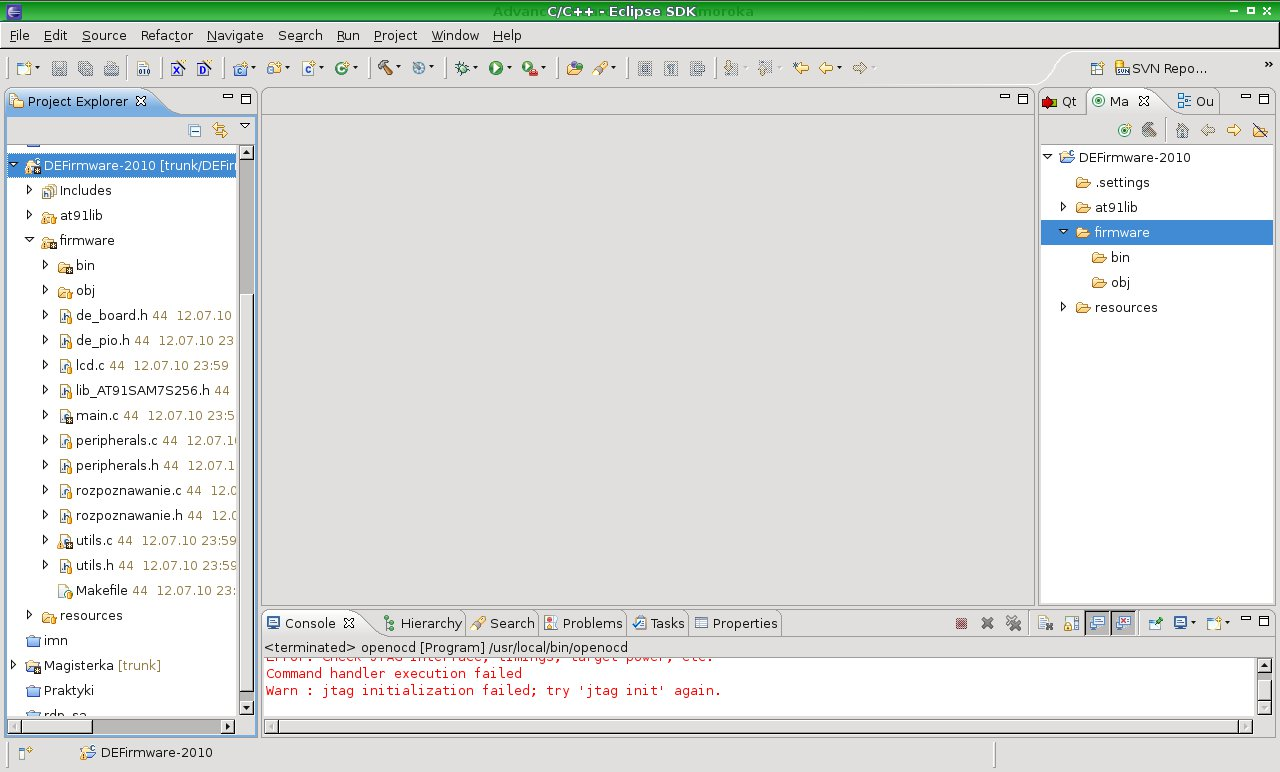
\includegraphics[width=150.0mm]{../images/ch03/Eclipse-MainWindow.jpg}
 \caption{Okno główne IDE Eclipse z dodanym projektem}
 \label{fig:Eclipse-MainWindow}
\end{figure}

\subsubsection{Dodawanie projektu z firmware'm Dark Explorer'a}
Do workspace'u Eclipse'a należy skopiować katalog z kodem sterującym robota.
Następnie dodajemy nowy projekt w IDE wybierając kolejno \textit{File --> New -->
C++ Project}. W oknie dialogowym \textit{C++ Project} (rysunek
\ref{fig:Eclipse-CPP-Project}), należy podać nazwę projektu która powinna być
zgodna z nazwą katalogu zawierającego kod robota. Następnie z listy Project type,
wybieramy \textit{Makefile project --> Empty Project}, a jako \textit{Toolchain}
wybieramy \textit{Other toolchain}. Całą operację zatwierdzamy przyciskiem
\textit{Finish}.

\begin{figure}[ht!]
 \centering
 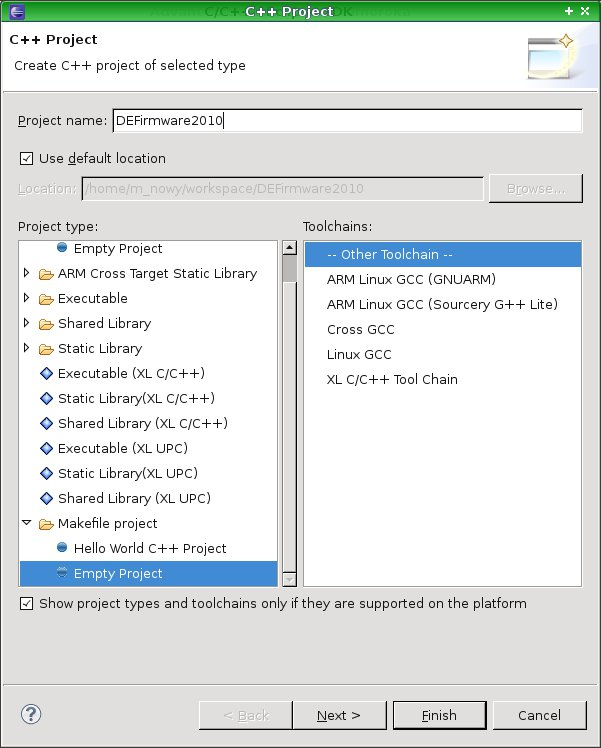
\includegraphics[height=100.0mm]{../images/ch03/Eclipse-CPP-Project.jpg}
 \caption{Okno dialogowe C++ Project}
 \label{fig:Eclipse-CPP-Project}
\end{figure}

Po poprawnym dodaniu projektu naszym oczom powinno się ukazać okno podobne do
tego na rysunku \ref{fig:Eclipse-MainWindow}

W przypadku gdy przed uruchomieniem Eclipse'a nie ustawiliśmy ścieżki do
odpowiedniego toolchain'a w zmiennych środowiskowych systemu. podjąć dodatkowe
kroki. Eclipse umożliwia konfigurowanie tych zmiennych dla pojedynczych
projektów. W celu ustawienia wymaganej ścieżki klikamy prawym klawiszem myszy na
nazwie naszego projektu w \textit{Project Explorer'ze} i wybieramy
\textit{Properties}.

\begin{figure}[ht!]
 \centering
 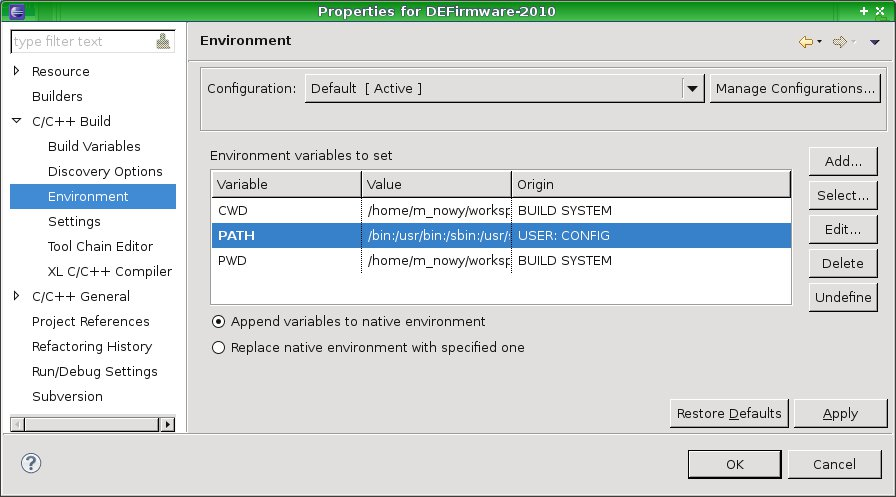
\includegraphics[width=150.0mm]{../images/ch03/Eclipse-Project-Properties.jpg}
 \caption{Okno dialogowe Properties}
 \label{fig:Eclipse-Project-Properties}
\end{figure}

Po ukazaniu się okna dialogowego \textit{Properties} (rysunek
\ref{fig:Eclipse-Project-Properties}) wybieramy \textit{C/C++ Build -->
Environment}. Następnie modyfikujemy zmienną \textit{PATH}, dodając na końcu
ścieżkę do naszego toolchain'a.

W celu przetestowania poprawności naszej konfiguracji możemy spróbować
skompilować kod, klikając prawym klawiszem myszy na nazwę projektu, a następnie
wybierając z menu kontekstowego opcję \textit{Build Project}. W wyniku powinniśmy
otrzymać dwa pliki binarne w katalogu \textit{firmware/bin}. Są to pliki gotowe
do umieszczenia w pamięci flash robota.

\subsection{Instalacja i konfiguracja toolchain'a}
W celu przetworzenia kodu do formy współpracującej z mikrokontrolerem ARM
niezbędny nam jest odpowiedni toolchain, czyli zestaw narzędzi generujących pliki
wykonywalne oraz pomagających w debugowaniu utworzonego oprogramowania. Tworzony
kod był kompilowany przy pomocy GNU ARM toolchain w wersji 3.4.3 dostępnej na
stronie
\url{http://www.gnuarm.com/bu-2.15_gcc-3.4.3-c-c++-java_nl-1.12.0_gi-6.1.tar.bz2}

Po ściągnięciu archiwum ze strony producenta należy rozpakować je do dowolnego
katalogu, na potrzeby tej pracy załóżmy że będzie to katalog \url{/usr/local/} W
celu zapewnienia dostępu do toolchain'a wszystkim programom wskazane jest
dodanie ścieżki /usr/local/bin do zmiennej środowiskowej PATH (komenda 
\verb|export PATH=$PATH:/usr/local/bin|).

W celu sprawdzenia poprawności instalacji należy wykonać komendę:
\begin{verbatim}
arm-elf-gcc --version 
\end{verbatim}
której wynikiem powinien być komunikat podobny do tego na rysunku \ref{fig:arm-elf-gcc-test}.

\begin{figure}
 \centering
 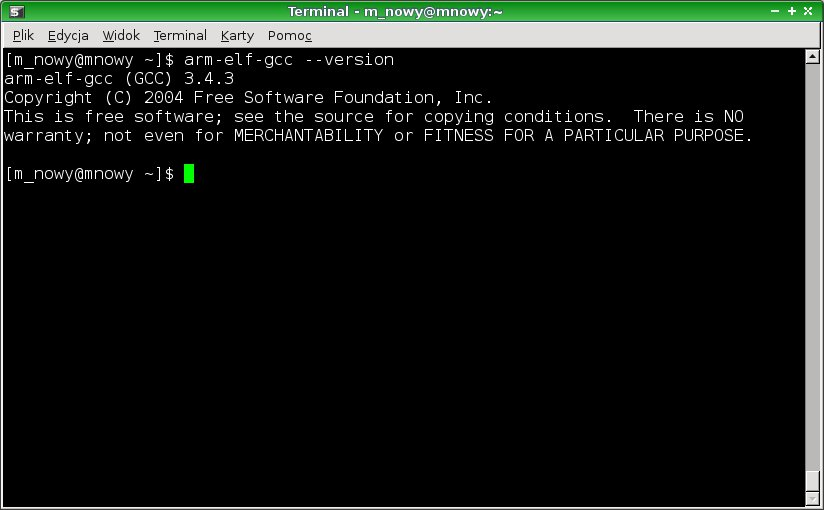
\includegraphics[width=150.0mm]{../images/ch03/arm-elf-gcc-test.jpg}
 \caption{Okno pokazujące odpowiedź prawidłowo zainstalowanego kompilatora}
 \label{fig:arm-elf-gcc-test}
\end{figure}

Trzeba wziąć pod uwagę to, iż toolchain o którym mowa był przygotowany pod system
32--bitowy. W przypadku konfiguracji na systemie 64--bitowym konieczne jest
zaopatrzenie się w 64--bitową wersje binarną toolchain'a lub skompilowanie go
samodzielnie. Ewentualne dodatkowe informacje można znaleźć pod adresem
\url{http://www.gnuarm.com}.

\subsection{Open On--Chip Debugger -- instalacja i konfiguracja}
\label{roz:opendocd-install}
Pamięć robota była programowana przy pomocy tego samego narzędzia które służy do
sprawdzania poprawności działania napisanego kodu. Mowa tu o oprogramowaniu Open
On--Chip Debugger.

Źródła programu należy pobrać ze strony:
\url{http://sourceforge.net/projects/openocd/}. Autorzy programu nie zamieścili
wersji binarnych, wiec kompilacje będziemy musieli przeprowadzić sami.

Po ściągnięciu i rozpakowaniu źródeł uruchamiamy skrypt configure z odpowiednimi
argumentami przy pomocy komendy:

\begin{verbatim}
./configure --prefix=/usr/local --enable-ft2232_libftdi 
\end{verbatim}

Dodatkowy argument powoduje włączenie obsługi urządzeń bazujących na układzie
FT2232 używając biblioteki libftdi. Jest to niezbędne przy korzystaniu z
programatora Triton JTAG A. W przypadku wykorzystywania programatora innej firmy
możliwa będzie konieczność wprowadzenia innego argumentu do skryptu
konfiguracyjnego. Argument prefix określa ścieżkę docelową instalacji
oprogramowania.

Gdy skrypt konfiguracyjny zakończy działanie z powodzeniem, możemy wywołać
komendę \verb|make && make install| w celu kompilacji i instalacji
oprogramowania.

Po zakończeniu powyższych czynności należy skopiować plik triton.cfg (dodatek \ref{chap:triton-cfg}) konfigurujący
połączenie przy pomocy programatora Triton JTAG A do katalogu
\url{/usr/local/openocd/interface}.

W celu przetestowania działania Open On--Chip Debugger'a należy podłączyć
programator Triton JTAG A do portu usb komputera oraz portu JTAG robota. Po
upewnieniu się że robot jest włączony wykonujemy komendę:

\begin{verbatim}
openocd -s /usr/local/share/openocd/scripts -f board/atmel_at91sam7s-ek.cfg
-f interface/triton.cfg 
\end{verbatim}

\begin{figure}[h!]
 \centering
 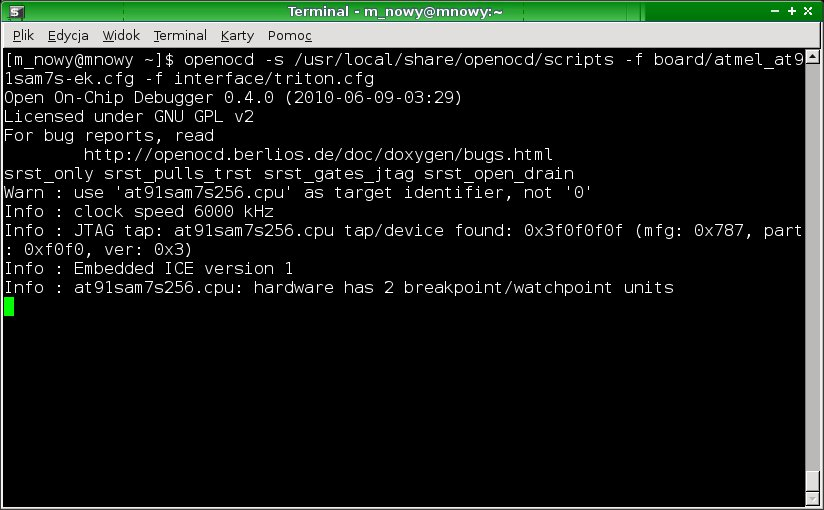
\includegraphics[width=150.0mm]{../images/ch03/openocd.jpg}
 \caption{Poprawnie uruchomiony openocd}
 \label{fig:openocd}
\end{figure}

\subsubsection{Programowanie pamięci Dark Explorer'a}
W celu wgrania programu do pamięci robota musimy uruchomić dwa narzędzia: telnet
oraz openocd. Procedura instalacji i uruchamiania openocd została opisana
wcześniej w rozdziale \ref{roz:opendocd-install}. W pierwszym kroku uruchamiamy
openocd w celu podłączenia się do robota. Następnie startujemy telnet za pomocą
polecenia:

\begin{verbatim}
 telnet localhost 4444
\end{verbatim}

Zapewnia nam to możliwość wysyłania komend sterujących do openocd. W celu
zaprogramowania pamięci flash Dark Explorer'a i uruchomienia nowej wersji
firmware'u należy wykonać zestaw komend:

\begin{verbatim}
 halt
 flash write_image {ścieżka_do_pliku_elf}
 reset init
 resume
\end{verbatim}

Natomiast w przypadku programowania pamięci RAM robota wykonujemy następujący
zestaw poleceń:

\begin{verbatim}
 halt
 load_image {ścieżka_do_pliku_bin} {początkowy_adres_pamięci}
 reset init
 resume
\end{verbatim}